\documentclass[ignorenonframetext,]{beamer}
\setbeamertemplate{caption}[numbered]
\setbeamertemplate{caption label separator}{: }
\setbeamercolor{caption name}{fg=normal text.fg}
\beamertemplatenavigationsymbolsempty
\usepackage{lmodern}
\usepackage{amssymb,amsmath}
\usepackage{ifxetex,ifluatex}
\usepackage{fixltx2e} % provides \textsubscript
\ifnum 0\ifxetex 1\fi\ifluatex 1\fi=0 % if pdftex
\usepackage[T1]{fontenc}
\usepackage[utf8]{inputenc}
\else % if luatex or xelatex
\ifxetex
\usepackage{mathspec}
\else
\usepackage{fontspec}
\fi
\defaultfontfeatures{Ligatures=TeX,Scale=MatchLowercase}
\fi
\usetheme{gcat}
% use upquote if available, for straight quotes in verbatim environments
\IfFileExists{upquote.sty}{\usepackage{upquote}}{}
% use microtype if available
\IfFileExists{microtype.sty}{%
\usepackage{microtype}
\UseMicrotypeSet[protrusion]{basicmath} % disable protrusion for tt fonts
}{}
\newif\ifbibliography
\usepackage{longtable,booktabs}
\usepackage{caption}
% These lines are needed to make table captions work with longtable:
\makeatletter
\def\fnum@table{\tablename~\thetable}
\makeatother
\usepackage{graphicx,grffile}
\makeatletter
\def\maxwidth{\ifdim\Gin@nat@width>\linewidth\linewidth\else\Gin@nat@width\fi}
\def\maxheight{\ifdim\Gin@nat@height>\textheight0.8\textheight\else\Gin@nat@height\fi}
\makeatother
% Scale images if necessary, so that they will not overflow the page
% margins by default, and it is still possible to overwrite the defaults
% using explicit options in \includegraphics[width, height, ...]{}
\setkeys{Gin}{width=\maxwidth,height=\maxheight,keepaspectratio}

% Prevent slide breaks in the middle of a paragraph:
\widowpenalties 1 10000
\raggedbottom

\AtBeginPart{
\let\insertpartnumber\relax
\let\partname\relax
\frame{\partpage}
}
\AtBeginSection{
\ifbibliography
\else
\let\insertsectionnumber\relax
\let\sectionname\relax
\frame{\sectionpage}
\fi
}
\AtBeginSubsection{
\let\insertsubsectionnumber\relax
\let\subsectionname\relax
\frame{\subsectionpage}
}

\setlength{\parindent}{0pt}
\setlength{\parskip}{6pt plus 2pt minus 1pt}
\setlength{\emergencystretch}{3em}  % prevent overfull lines
\providecommand{\tightlist}{%
\setlength{\itemsep}{0pt}\setlength{\parskip}{0pt}}
\setcounter{secnumdepth}{0}

\title{Statistically significant SNP combinations for GWAS data}
\author{Xavier Duran\\
GCAT Genomes for Life\\
Institut de Recerca Germans Trias i Pujol (IGTP)}
\date{Bioinfo Talks\\
February 15\textsuperscript{th} 2017}

\begin{document}
\frame{\titlepage}

\begin{frame}{Missing heritability problem on GWAS}

GWAS studies have discovered many loci associated with various complex
traits but they only explain a very small part of the human heritability

Screening of individual SNPs using statistical tests to assess the
association of each SNP with a phenotype

\end{frame}

\begin{frame}{Statistical epistatic interactions are hard to find}

This unexplained variation because GWAS tries to solve common variant,
common disease hypothesis

Most complex traits are due to the effect of interactions of different
SNP

Combinatorial effects of multiple SNPs

Epistasis can be part of the explanation

\end{frame}

\begin{frame}{Why?}

Apply data mining and machine learning techniques to biological data
analysis

Hard computational problem

GCAT

\end{frame}

\begin{frame}{Limitless arity multi-testing procedure (LAMP)}

Computational complexity

Statistical significance

\end{frame}

\begin{frame}{Outline}

The complexity of combinatorial variant discovery

How does LAMP approaches a solution

Results on a lung cancer dataset

\end{frame}

\begin{frame}{Finding combinations of features}

\begin{block}{Computational problem}

Exploring all combinations is computationally prohibitive

Exponential growth: for \(M\) binary variables, \(2^M\) tests computed

\end{block}

\end{frame}

\begin{frame}{Finding combinations of features}

\begin{block}{Statistical problem}

Discovered combinations are statistically unlikely due to multiple
testing correction

For \(M\) binary variables, Bonferroni correction sets significance
below \(\frac{\alpha}{2^M}\)

\end{block}

\end{frame}

\begin{frame}{Finding combinations of features}

\begin{block}{We cannot test all combinations}

Most machine learning methods (RF) don't evaluate statistical
significance of the reported results

Too much false positives, very costly to futher explore hypothesis

Not comprehensive

\end{block}

\end{frame}

\begin{frame}{Limitless arity multi-testing procedure (LAMP)}

Multiple testing procedure for listing ALL statistically significant
high order interactions

\end{frame}

\begin{frame}{Limitless arity multi-testing procedure (LAMP)}

\begin{block}{Testable combinations}

Upper bound of Family Wise Error Ratio (FWER)

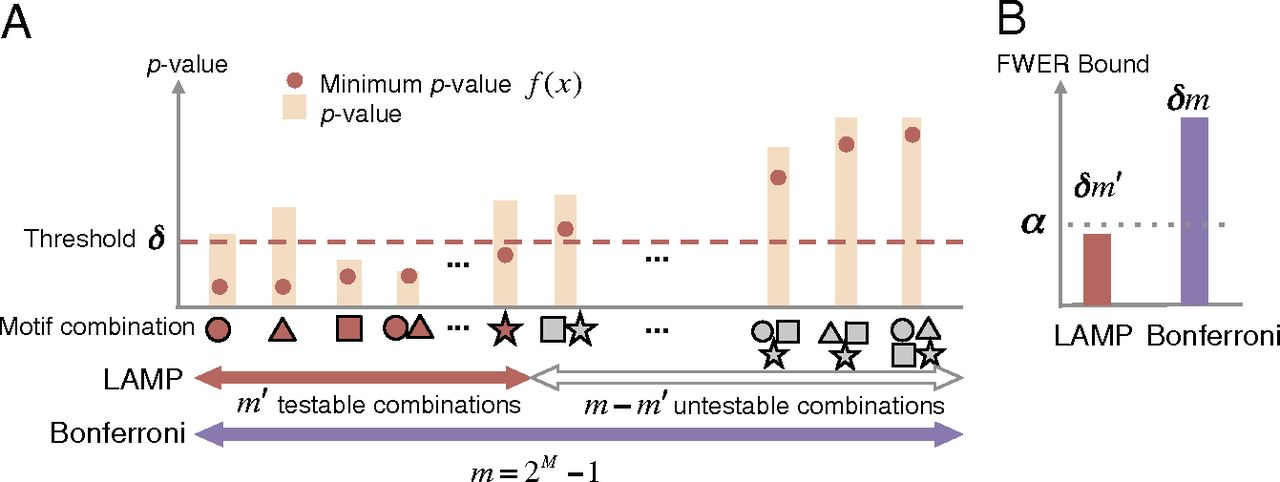
\includegraphics{images/F2.large.jpg}

{[}Terada et al. 2013{]}

\end{block}

\end{frame}

\begin{frame}{Limitless arity multi-testing procedure (LAMP)}

\begin{block}{Fisher's exact test}

Not all combinations are frequent enough to become frequent in any
case/control setting

Each combination has a maximum p-value, independent of its distribution
on the two classes

Test only what is relevant to test

\begin{longtable}[]{@{}llll@{}}
\toprule
& Case & Control & Total\tabularnewline
\midrule
\endhead
Has \(S_i\) & 171 & 206 & 377\tabularnewline
Hasn't \(S_i\) & 29 & 94 & 123\tabularnewline
total & 200 & 300 & 500\tabularnewline
\bottomrule
\end{longtable}

\end{block}

\end{frame}

\begin{frame}{Limitless arity multi-testing procedure (LAMP)}

\begin{block}{Fisher's exact test}

Not all combinations are frequent enough to become frequent in any
case/control setting

Each combination has a maximum p-value, independent of its distribution
on the two classes

Test only what is relevant to test

\begin{longtable}[]{@{}llll@{}}
\toprule
& Case & Control & Total\tabularnewline
\midrule
\endhead
Has \(S_i\) & k & K-k & K\tabularnewline
Hasn't \(S_i\) & n-k & N-K-n+k & N-K\tabularnewline
total & n & N-n & N\tabularnewline
\bottomrule
\end{longtable}

\end{block}

\end{frame}

\end{document}
